\documentclass[12pt]{article}

\usepackage[margin=1in]{geometry}
\usepackage{amsmath,amsthm,amssymb}
\usepackage{hyperref}
\usepackage{xcolor}
\usepackage{graphicx}

\begin{document}

\title{CS484: Parallel Programming - Spring 2017 \\
MP2 \\
Due Date : Monday, March 20, 11:59PM \\
Submission Method : SVN}

\maketitle

\section {Assignment}

\subsection{Queue Implementation}

Implement a lock-free circular queue using c++11 atomics, that can support multiple producers and consumers.
Compare the performance of your implementation against an equivalent version that
uses locks for synchronisation. You will be using the c++ interface to pthreads for this assignment.

The queue should support the following functions :

\begin{itemize}
\item Insert an element
\item Delete an element
\item Check if the queue is full
\item Check if the queue is empty
\end{itemize}	


Answer the following questions :

\begin{itemize}
\item What are the atomics you used for your implementation and why?
\item Do the following experiments with your implementation :
  \begin{itemize}
  \item For a fixed number of insertions and deletions, measure the performance of the two implementations for varying number of threads
 \item For a fixed number of threads, measure the performance of the two implementations by varying the total number of insertions and deletions
  \end{itemize}

\item Tabulate your results and plot graphs for both experiments. Clearly indicate the parameters, i.e total number of operations (insertions and deletions) and the number of threads.
You have to perform all your experiments on Taub.
\end{itemize}

We have provided you with starter code for both versions, you can find it under the folder $queue$ in the MP2\_new directory once you extract the tar file.
Here is a good reference for multi-producer, multi-consumer queues with pseudo code
\url{https://www.research.ibm.com/people/m/michael/podc-1996.pdf}

Here is a link to the list of c/c++11 atomics, that might be useful to you.

\url{http://en.cppreference.com/w/cpp/atomic}


\subsection{Parallelizing WaTor}


For this MP, you will be using MPI to implement a parallel WaTor simulation. WaTor is a population dynamics simulation implemented on a 2D toroidal (wrap-around) grid; for more information, see \href{https://en.wikipedia.org/wiki/WaTor}{here}.


We have provided you with a reference sequential implementation in ``wator.cpp'', under the folder $wator$ which includes support functions. In \textit{main()}, there are calls to \textit{wator()} and \textit{wator\_parallel()}. \textit{wator()} runs the sequential version of the Wator simulation, and is fully-functional. \textit{wator\_parallel()} contains the same code as \textit{wator()}, but the calls to \textit{update\_sharks()} and \textit{update\_fish()} are replaced by \textit{update\_sharks\_in\_parallel()} and \textit{update\_fish\_in\_parallel()} respectively.

Your task is to write the program for \textit{update\_sharks\_in\_parallel()} and \textit{update\_fish\_in\_parallel()}, using the sequential versions of the methods as references. You should make use of MPI's message passing features to add parallelism to the update methods.
The sequential program discretizes the domain into cells, which contain sharks and fish. The locations of sharks and fish are updated in a doubly nested loop based on the
contents of its neighboring cells.
For the parallel version, you can divide the domain into blocks/tiles with each tile consisting of a number of rows and columns. You can assign a tile to an MPI process.
During an update phase, the elements of a tile will need rows and columns from its four nearest neighbors - north, south, east and west.
For your convenience, you can assume the domain is toroidal where the cells wrap around, i.e the northern neighbor of row 0, lies on row N-1, for an NXN domain. Similarly, the western neighbor of column 0, lies on column N-1.

\begin{figure}
\caption{Section of a Wator world (green=fish, red=shark, blue-water)}
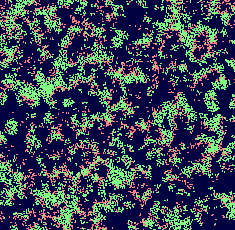
\includegraphics[scale=1.0]{wator.png}
\centering
\end{figure}

You have to implement the following versions :

\begin{itemize}
\item Perform nearest neighbor exchange using blocking send/receive, preferrably MPI\_SendRecv (single call that exchanges messages between a communicating pair).
\item Use non-blocking MPI calls (MPI\_Irecv and MPI\_Isend) for nearest neighbor exchange
\end{itemize}

For each version, do strong scaling experiments by changing the number of MPI processes, fixing the size of the mesh (NXN) and the number of iterations.
Measure the time taken for each experiment and plot a graph using the sequential time as baseline.
Explain your parallelization strategy and compare it with the results you obtained.


Verify your implementation is correct by comparing the number of fish and sharks per chronon to the reference implementation (the algorithm is completely deterministic). Test your code locally first, then on Taub using a batch script (please avoid using Taub's login nodes).

It should not be necessary to edit any methods other than \textit{update\_sharks\_in\_parallel()}, \textit{update\_fish\_in\_parallel()}, and \textit{main()}, though you are free to edit the rest of wator.cpp as you see fit. You will also need to add includes for MPI. Feel free to edit any of the constants at the top of wator.cpp to vary the parameters of your world. You may also find it useful to comment / uncomment the \textit{\#define ASCII\_ART} line at the top of the file to toggle printing a snippet of the Wator world to your terminal.

\subsection{Submission}

Submission is via svn. Create a folder in your svn account named ``MP2''. Please have separate folders for each section - list implementation and Wator. The folders should contain all the files necessary for executing your code, \textbf{including makefiles and instructions for compiling / running}. You should also submit a neatly typed report, preferrably in pdf, which contains the graphs and analyses of your results.

\end{document}
